\documentclass[12pt, a4paper]{article}

% --- Language & Encoding ------------------------------------------------------
\usepackage[english]{babel}
\usepackage[T1]{fontenc}
\usepackage[utf8]{inputenc}

% --- Page Layout --------------------------------------------------------------
\usepackage[
  a4paper,
  top=2.5cm,
  bottom=2.5cm,
  left=3cm,
  right=3cm,
  marginparwidth=1.75cm
]{geometry}

% --- Typography ---------------------------------------------------------------
\usepackage{lmodern}
\usepackage{microtype}
\usepackage{setspace}
\onehalfspacing

% --- Mathematics --------------------------------------------------------------
\usepackage{amsmath}
\usepackage{amssymb}

% --- Graphics & Figures -------------------------------------------------------
\usepackage{graphicx}
\usepackage[labelfont=bf, font=small, skip=6pt]{caption}
\usepackage{float}
\usepackage{subcaption}

% --- Tables -------------------------------------------------------------------
\usepackage{booktabs}
\usepackage{array}
\usepackage{tabularx}
\newcolumntype{Y}{>{\raggedright\arraybackslash}X}
\newcolumntype{P}[1]{>{\raggedright\arraybackslash}p{#1}}
\usepackage{xcolor}
\usepackage{colortbl}
\usepackage{multirow}

% --- Headers & Footers --------------------------------------------------------
\usepackage{fancyhdr}
\pagestyle{fancy}
\fancyhf{}
\setlength{\headheight}{14pt}
\renewcommand{\headrulewidth}{0.4pt}
\fancyhead[L]{\small\textit{PSG College of Technology}}
\fancyhead[R]{\small\textit{Tasklet Scheduling Project}}
\fancyfoot[C]{\thepage}

% --- Section Formatting -------------------------------------------------------
\usepackage{titlesec}
\titleformat{\section}{\large\bfseries}{{\thesection}}{1em}{}[\titlerule]
\titleformat{\subsection}{\normalsize\bfseries}{{\thesubsection}}{1em}{}
\titlespacing*{\section}{0pt}{16pt}{8pt}
\titlespacing*{\subsection}{0pt}{10pt}{4pt}

% --- Hyperlinks ---------------------------------------------------------------
\usepackage[
  colorlinks=true,
  linkcolor=blue!70!black,
  citecolor=blue!70!black,
  urlcolor=blue!70!black
]{hyperref}

% --- Miscellaneous ------------------------------------------------------------
\usepackage{parskip}
\usepackage{listings}
\usepackage{placeins}
\setlength{\parskip}{6pt}
\setlength{\emergencystretch}{2em}
\usepackage{enumitem}

% --- Color Definitions --------------------------------------------------------
\definecolor{headerblue}{RGB}{36, 74, 116}
\definecolor{rowgray}{RGB}{240, 240, 240}
\definecolor{tpgreen}{RGB}{198, 239, 206}
\definecolor{tnblue}{RGB}{197, 217, 241}
\definecolor{fpred}{RGB}{255, 199, 206}
\definecolor{fnyellow}{RGB}{255, 235, 156}
\graphicspath{{figures/}}

\newcommand{\maybeincludegraphics}[2][]{%
  \IfFileExists{#2}{\includegraphics[#1]{#2}}{\fbox{\parbox[c][2.8cm][c]{4.5cm}{\centering Logo}}}%
}

\lstset{basicstyle=\ttfamily\footnotesize,breaklines=true,columns=fullflexible,keepspaces=true,frame=single,backgroundcolor=\color{rowgray},aboveskip=10pt,belowskip=10pt}


\hypersetup{
  pdftitle={Tasklet Scheduling for Pipeline-Parallel LLM Training on Heterogeneous WANs},
  pdfauthor={Dhaarun Abhimanyu S; Karthick J S; Mohana Kumar P; Sanjeev M S; Surya Narayanaa N T},
  pdfsubject={PSG College of Technology project implementation and progress report},
  pageanchor=false
}

\begin{document}

% The layout, typography, section sequence and front matter follow the supplied template.
\begin{titlepage}
  \thispagestyle{empty}
  \centering
  \vspace*{0.15cm}
  
\includegraphics[width=6.2cm,keepaspectratio]{psg_tech_logo.png}\\[0.35cm]
  {\Large\bfseries PSG College of Technology}\\[0.25em]
  {\large Department of Computer Science and Engineering}\\[0.15em]
  {\normalsize Coimbatore, Tamil Nadu}

  \vspace{0.4cm}
  \rule{0.85\textwidth}{0.5pt}
  \vspace{0.55cm}
  {\large\bfseries PROJECT REPORT}
  \vspace{0.55cm}

  {\LARGE\bfseries Tasklet Scheduling for\\[0.25em]
  Pipeline-Parallel LLM Training\\[0.25em]
  on Heterogeneous WANs}

  \vspace{0.55cm}
  {\itshape Implementation, Validation and Project Progress}
  \vspace{0.45cm}

  \begin{tabularx}{0.88\textwidth}{>{\bfseries}l >{\raggedright\arraybackslash}X}
    Project Area: & Distributed training, heterogeneous computing and adaptive scheduling\\
    Baseline: & Decentralized Training of Foundation Models (DT-FM)\\
    Reporting Date: & 4 October 2026
  \end{tabularx}

  \vspace{0.8cm}
  \begin{minipage}[t]{0.61\textwidth}
    \raggedright
    \textbf{Submitted by:}\\[0.4em]
    \begin{tabular}{@{}ll@{}}
      Dhaarun Abhimanyu S & 23N216\\[0.25em]
      Karthick J S & 23N221\\[0.25em]
      Mohana Kumar P & 23N228\\[0.25em]
      Sanjeev M S & 23N248\\[0.25em]
      Surya Narayanaa N T & 23N256
    \end{tabular}
  \end{minipage}
  \hfill
  \begin{minipage}[t]{0.35\textwidth}
    \raggedleft
    \textbf{Project Guide:}\\[0.4em]
    {\large\bfseries Dr.\ Jayashree L S}\\[0.35em]
    Department of Computer Science and Engineering\\
    PSG College of Technology
  \end{minipage}

  \vfill
  \rule{0.85\textwidth}{0.5pt}\\[0.3cm]
  {\large October 2026}
\end{titlepage}

\pagenumbering{roman}
\thispagestyle{fancy}
\vspace*{0.16\textheight}
\begin{center}
  {\Large\bfseries Acknowledgement}
\end{center}
\vspace{0.7cm}

We express our sincere gratitude to Dr.\ Jayashree L S, Department of Computer Science and Engineering, PSG College of Technology, for her guidance and support for the project \textit{``Tasklet Scheduling for Pipeline-Parallel LLM Training on Heterogeneous WANs.''}

We thank the Department of Computer Science and Engineering and PSG College of Technology for the academic environment in which this project is being developed. We also acknowledge the contributions of our project team in reproducing the training baseline, extending device support, developing scheduling and measurement tools, and preparing repeatable experimental workflows.

We acknowledge the authors and maintainers of DT-FM for releasing their research implementation, which serves as the foundation for our work. The PyTorch, MLflow and related open-source communities provide the software infrastructure used by the prototype. The distinction between inherited functionality and our extensions is maintained throughout this report.

\vspace*{\fill}
\newpage

\begin{abstract}
\noindent
This project investigates how underused laptops and workstations can participate in pipeline-parallel model training despite differences in compute capability, memory capacity and network connectivity. The work extends the open-source Decentralized Training of Foundation Models (DT-FM) implementation with portable execution paths, CPU-staged heterogeneous communication, network and compute profiling, resource-aware layer allocation, transactional layer migration, experiment tracking and reproducible deployment.

The current prototype supports CPU training and device-specific paths for NVIDIA CUDA, AMD ROCm, Intel XPU and Intel UHD DirectML. Static scheduling combines a network-derived pipeline order with capacity-constrained layer allocation; dynamic scheduling measures available memory and compute speed before constructing the stages. Optional periodic rebalancing transfers trained layers and supported SGD state at completed optimizer-step boundaries. Per-rank JSON measurements, optional MLflow tracking and an automated lab workflow make training behavior and experimental scope visible.

The repository contains 36 team commits beyond its original upstream baseline. The latest published continuous-integration run passed all 61 tests, CPU smoke training, training across two containers and the MLflow demonstration; the CUDA image build also passed. Recorded development validation includes local CPU/AMD and CPU/Intel UHD pipelines and CPU/Gloo migration-continuity checks. These results establish a working and testable prototype. Physical multi-host WAN validation, GPU migration, measured scheduling speedup and end-to-end model-quality evaluation remain outstanding. Automatic recovery from a crashed training worker and communication compression are retained as proposed extensions, rather than reported as completed capabilities.
\end{abstract}

\newpage
\begingroup
\setstretch{1.05}
\small
\tableofcontents
\endgroup
\newpage
\pagenumbering{arabic}
\hypersetup{pageanchor=true}

% =============================================================================
\section{Problem Definition}
% =============================================================================

The Review 1 presentation identifies a practical mismatch: advanced model training requires substantial computing resources, while consumer GPUs, workstations and institutional computers can remain underused. Pooling these machines could make experimentation more accessible, but the resulting environment differs from a tightly coupled training cluster. Devices may have different accelerator vendors, memory capacities and compute rates; their network links may have unequal latency and bandwidth; and their availability can change during a run.

The project studies the systems problem of assigning and executing training work across such resources. Pipeline parallelism divides a model into stages, while microbatches pass through these stages during forward and backward computation. A useful allocation must fit each participating device, avoid excessive imbalance between stages and account for communication between neighboring ranks. The original DT-FM research and code provide the baseline for investigating this setting \cite{dtfm}.

\subsection{Project Objective}

The principal objective is to develop and evaluate an adaptive orchestration prototype for pipeline-parallel training on heterogeneous machines. The implemented work addresses the following goals:
\begin{itemize}[leftmargin=1.2cm,itemsep=3pt]
  \item reproduce the original training path on accessible local hardware;
  \item permit pipeline stages to use different supported compute devices;
  \item measure communication, compute performance and available memory;
  \item generate consistent rank commands and contiguous layer assignments;
  \item adjust layer allocation at startup and optionally between training steps;
  \item preserve trained state when a live rank transfers layers to another rank;
  \item expose per-rank execution and failure status through measurable artifacts; and
  \item provide repeatable lab comparisons and portable deployment tools.
\end{itemize}

The Review 1 proposal additionally targets recovery from worker loss and communication compression. Those objectives motivate the wider design, but the current implementation does not yet satisfy them. A successful migration between live workers is different from recovery after a worker has disappeared.

\subsection{Research Questions}

The project is organized around four questions. First, can the same pipeline code execute correctly across commodity device types without a common GPU collective backend? Second, can measured resources determine a feasible and reproducible model partition? Third, can the partition change without losing trained parameters or supported optimizer state? Finally, does resource-aware allocation improve measured end-to-end performance over equal allocation on physical heterogeneous hosts?

The first three questions have implementation and local validation evidence. The fourth requires controlled physical-host experiments. This report therefore separates functional correctness from performance benefit and model quality.

\subsection{Tasklets, Stages and Heterogeneity}

The term \textit{tasklet} comes from the baseline research's allocation of training work. In our current extension, the movable ownership unit is a transformer layer within a contiguous pipeline stage. A process or \textit{rank} owns its assigned stage. The first rank additionally owns input embeddings, and the last rank owns the classification head. Layer counts may differ, but every participating rank receives at least one transformer layer.

The implementation does not provide arbitrary GPU-kernel tasklet scheduling. It also does not implement mixed-vendor GPU collectives. Heterogeneous execution is achieved by staging boundary activations and gradients through CPU tensors and transporting them with Gloo, while each rank performs its local model computation on its selected device.

\subsection{Scope and Evidence Boundary}

The main report describes the committed DT-FM extension through commit \texttt{e0c0507}, dated 4 October 2026. The original upstream baseline is \texttt{cda948f}, dated 3 July 2022. Our team's first recorded extension is dated 17 August 2026. The presentation provides the project title, membership, motivation, proposed system design and planned timeline; repository code, documentation and CI provide implementation evidence \cite{upstream,fork,ci}.

The primary reproducible workloads are small synthetic classification models and a fixed subset of Quora Question Pairs (QQP). BERT-style parameter presets are supplied, but the code's profile name does not imply that a pretrained BERT model is being fine-tuned. The reported smoke results are not a foundation-model training benchmark or an accuracy result. A newer Tamil summarization extension present in the working directory is described separately as ongoing work.

% =============================================================================
\section{Methodology}
% =============================================================================

\subsection{Literature Survey}

Three studies identified in Review 1 guide the design. DT-FM examines communication-aware placement of training work across decentralized heterogeneous resources \cite{dtfm}. We use its released pipeline and data-parallel code as the inherited foundation and extend the operational workflow and allocation mechanisms.

ReCycle studies resilience through microbatch rerouting to surviving data-parallel peers and adaptive use of pipeline slack \cite{recycle}. It informs the proposed recovery direction. Our current fixed-membership pipeline does not implement this rerouting or inherit ReCycle's failure tolerance.

Deep Gradient Compression studies sparse gradient communication with supporting mechanisms to preserve training behavior \cite{dgc}. It motivates reducing network traffic in future work. The current CPU-staged pipeline sends boundary tensors without implementing that compression method; gradient sparsification for data-parallel synchronization also differs from compressing pipeline activations.

\begin{table}[H]
\centering\small
\caption{Literature roles and their relationship to the prototype.}
\begin{tabularx}{\textwidth}{P{2.3cm}YY}
\toprule
\textbf{Study} & \textbf{Design relevance} & \textbf{Current relationship}\\
\midrule
DT-FM, 2022 & Communication-aware assignment and decentralized training. & Baseline implementation; our extensions add portable execution, allocation and measurement tools.\\
ReCycle, 2024 & Training continuity under worker failures. & Literature direction for future recovery; not an implemented recovery subsystem.\\
Deep Gradient Compression, 2018 & Reducing gradient communication traffic. & Candidate communication optimization; not enabled in the current pipeline.\\
\bottomrule
\end{tabularx}
\end{table}

\subsection{Repository and Development Workflow}

The original repository contains research-oriented training modules, data-parallel implementations, pipeline code, an evolutionary scheduler and AWS/network-experiment scripts. These are inherited assets. Our team first added local setup, data download, a complete one-stage model path and executable GPipe/QQP smoke tests. Subsequent work broadened hardware support and connected profiling, scheduling, tracking and deployment to actual training commands.

The comparison is based on shared Git ancestry rather than repository names. There are 36 team commits after the original upstream baseline. Excluding whitespace-only differences, the comparison touches 98 files. Large raw insertion totals are not used as an implementation metric because the tree includes a tokenizer vocabulary and line-ending changes. The contribution summary is based on behavior, modules and validation rather than lines of code.

Work is grouped into five stages: reproduce the baseline, make execution portable, instrument the runtime, add allocation and migration, and package repeatable experiments. Each stage is supported by specific scripts, modules and checks rather than by a numerical completion percentage.

\subsection{Hardware and Software Configuration}

CPU is the portable distributed baseline. Device helpers identify CUDA, ROCm and XPU runtimes and enforce explicit selection where required. An explicit unavailable device produces an error; automatic selection can fall back to CPU. DirectML selection remains explicit because a hybrid laptop may expose both NVIDIA and Intel adapters.

\begin{table}[H]
\centering\small
\caption{Execution paths and recorded verification scope.}
\begin{tabularx}{\textwidth}{P{2.05cm}YY}
\toprule
\textbf{Path} & \textbf{Execution arrangement} & \textbf{Evidence / restriction}\\
\midrule
CPU & Windows/Linux/WSL; local ranks and Gloo pipelines. & Development checks and latest Docker CI cover real forward, backward and optimizer steps.\\
NVIDIA CUDA & Native legacy setup or CUDA Docker target. & Original local reproduction retained. Latest CI builds the image without GPU execution.\\
AMD ROCm & Device-specific runtime; CPU-staged Gloo for multiple stages. & Recorded Radeon 860M single-process and mixed CPU/AMD local training.\\
Intel XPU & Supported Intel runtime; FP32 and pipeline-only Gloo. & Implemented; supported-hardware execution remains to be verified.\\
Intel UHD DirectML & Separate Python 3.11 environment under WSL; explicit adapter. & Recorded single-process and mixed CPU/Intel UHD training. Automatic free-device-memory discovery is unavailable.\\
\bottomrule
\end{tabularx}
\end{table}

The presentation's original software requirements describe the initial CUDA reproduction stack. Later device paths use separate environments, and the published Docker baseline uses Python 3.10 and PyTorch 2.8.0. The CUDA target uses CUDA 12.6.3 and CuPy 13.6.0. These configurations should not be mixed by sourcing the legacy CUDA environment inside the newer container. Native vendor setup and container setup are documented independently.

\subsection{Implemented System Architecture}

The runtime has three related paths. A measurement path gathers network observations and device compute/memory reports. A planning path converts those observations into rank order and stage counts. A training path executes the negotiated stages and emits metrics. Optional rebalancing repeats resource planning at a safe boundary, while the lab coordinator runs controlled trials and collects their artifacts.

\begin{figure}[H]
\centering
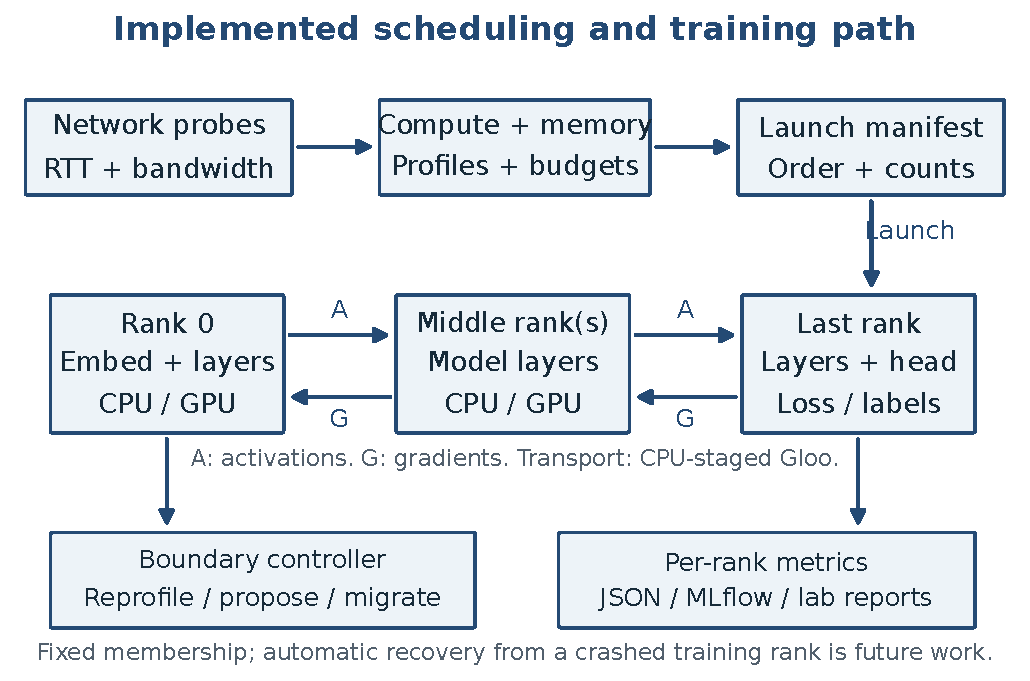
\includegraphics[width=\textwidth]{implemented_architecture.pdf}
\caption{Current implementation: measured allocation, CPU-staged pipeline transport, optional live-rank migration and per-rank observability.}
\label{fig:implemented}
\end{figure}

Training membership stays fixed. Resource discovery can change the number of layers assigned to a rank, but it does not add or remove ranks. The common configuration is pipeline-only GPipe with data-group size one and FP32. Model dimensions, batch settings, vocabulary and scheduling policy must agree across ranks before model construction.

\subsection{Review 1 Design and Planned Recovery}

Figures~\ref{fig:proposal} and~\ref{fig:recovery} reproduce the supplied presentation's design. They show the broader intended combination of tasklet assignment, data-parallel groups, pipeline structures, communication compression, liveness monitoring and redistribution after failure. These diagrams describe the proposal, not a claim that every box has been implemented.

The present prototype supplies portable training, measurement, layer allocation and transfers between live pipeline workers. It does not provide the proposed failure monitor, redundant data-parallel recovery or compressed pipeline transport. In particular, rollback of a candidate stage is possible only while the participating ranks remain alive and can communicate.

\begin{figure}[H]
\centering
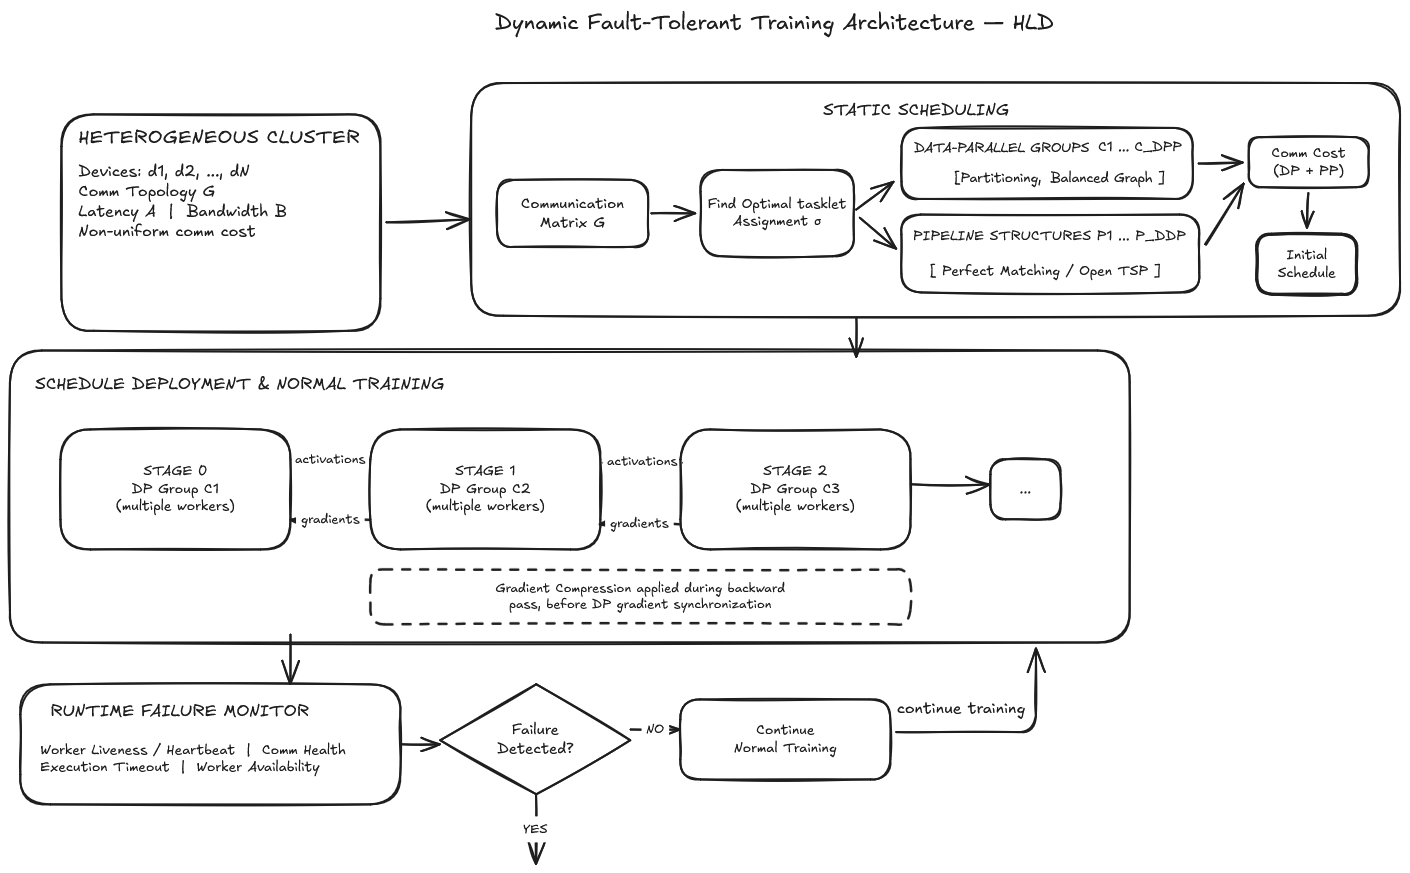
\includegraphics[width=\textwidth]{proposed_architecture.png}
\caption{Broader proposed architecture from Review 1. Failure monitoring and compression are future extensions.}
\label{fig:proposal}
\end{figure}

\begin{figure}[H]
\centering
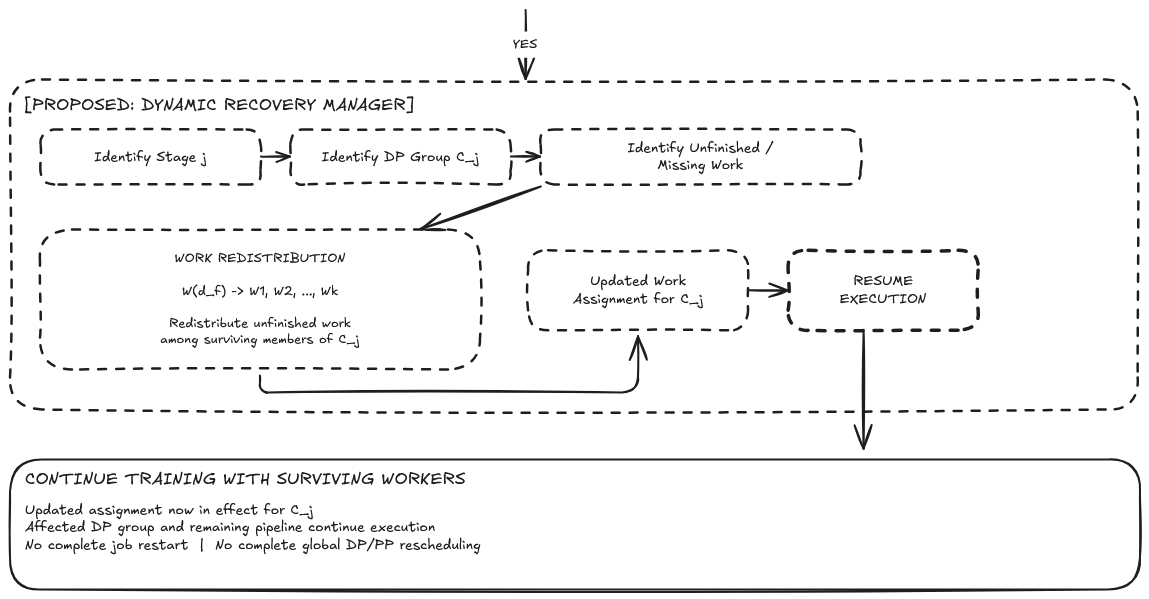
\includegraphics[width=\textwidth]{proposed_recovery.png}
\caption{Proposed recovery manager from Review 1. Worker-loss redistribution without restarting training is not implemented in the current fixed-membership runtime.}
\label{fig:recovery}
\end{figure}

\subsection{Communication Probing and Rank Ordering}

Each probe source records observations for its peers. The aggregation code preserves source-directed measurements, verifies rank identifiers and emits the same matrices on all ranks. Off-diagonal failures are represented by JSON \texttt{null}; only self-links are zero. If a probe listener cannot start, usable observations from other pairs are retained. This does not recover a failed training process group.

Latency is a measured round-trip time. Bandwidth is an echo-based estimate calculated using half the round-trip duration. These values do not isolate one-way WAN capacity or accelerator-transfer cost. A profile therefore supports a ranking proxy rather than a calibrated prediction of total training time.

For payload size $P$ bytes, RTT $R_{ij}$ milliseconds and estimated bandwidth $B_{ij}$ megabits per second, the manifest adapter uses the bidirectional edge proxy
\[
  c(i,j)=\sum_{(a,b)\in\{(i,j),(j,i)\}}
  \left(R_{ab}+\frac{8P}{1000B_{ab}}\right).
\]
An edge is unavailable if either direction lacks a measurement. The adapter selects the minimum-cost path visiting every measured rank, with deterministic tie breaking. Its Held--Karp path search has $O(K^2 2^K)$ complexity for $K$ ranks; manifest validation limits profiles to 2--12 ranks. It then emits explicit host, device, master address and rank commands. The original measured-rank identity remains available after reordering.

\subsection{Compute Profiling and Static Layer Allocation}

The compute profiler measures a transformer layer's forward, backward and SGD work under the intended model and batch configuration. It also measures endpoint overhead for embeddings and the classification head. An operator supplies a maximum layer count for each rank, with memory headroom reserved for activations and endpoints. A profile is valid only when its device identity and model dimensions match the launch.

For a fixed network-derived order, let $n_r$ be the layer count, $t_r$ the measured per-layer compute time, $h_r$ the endpoint overhead and $u_r$ the supplied layer limit. The static planner solves the following estimated bottleneck objective:
\[
  \min_{n_0,\ldots,n_{K-1}}\max_r(n_rt_r+h_r)
  \quad\text{subject to}\quad
  \sum_r n_r=L,\qquad 1\leq n_r\leq u_r.
\]
It searches the finite set of candidate stage times and chooses a deterministic minimax allocation. This is optimal for the stated compute estimate and fixed order, not for the full system's throughput. Communication, synchronization and pipeline effects can change the observed result.

Assignments use contiguous half-open layer ranges. For example, counts $[1,3,2]$ describe six layers with ranges $[0,1)$, $[1,4)$ and $[4,6)$. This is an illustrative valid partition, not a measured claim that this split is faster on the team's machines.

\subsection{Live Resource Discovery and Dynamic Allocation}

Dynamic startup discovers current resources instead of embedding a stale compute snapshot in the manifest. Ranks first agree on the workload and policy, check minimal feasibility, calibrate computation, sample memory again and derive a common allocation. The resulting plan is saved per rank and included in metrics.

Windows host discovery uses the smaller of available physical RAM and commit headroom. Linux reads \texttt{MemAvailable} and bounds it by visible cgroup headroom. Accelerator discovery uses the runtime's free-memory API when available. DirectML fails explicitly in this mode because a supported free-device-memory query is absent; static scheduling remains available for DirectML.

For a resource pool $p$ with available memory $A_p$, the default budget is
\[
  Q_p=\max\left(0,\left\lfloor0.7A_p\right\rfloor-256\,\mathrm{MiB}\right).
\]
The model combines exact FP32 parameter/gradient element counts with estimates for retained activations, attention workspace, endpoints and communication buffers, padded by 25\%. It is not a measured peak-memory guarantee or a reservation of the operating system's memory.

Ranks sharing a physical host consume one host budget. Accelerator ranks sharing a device identity consume one device budget. When a runtime cannot expose a UUID, the grouping is conservative. Containers on the same host must supply a shared scheduler host identity so that their separate container hostnames do not duplicate the available RAM.

The dynamic allocator first gives each rank one layer. Each remaining layer goes to the eligible rank with the smallest resulting estimated compute time, subject to all shared budgets. If the model cannot fit, the launch fails before construction rather than silently reducing the total number of layers or dropping a rank. This greedy policy is deterministic; it is not an end-to-end global throughput optimizer.

\subsection{Periodic Rebalancing and Transactional Migration}

Rebalancing is optional and disabled by default. When enabled, all ranks reach a completed optimizer-step boundary with the pipeline drained. The controller profiles compute again, samples memory and proposes a new partition. By default the proposal must reduce the estimated bottleneck by at least 10\%, unless the current partition exceeds the new estimated memory budgets. Migration overhead is not part of that improvement estimate.

\begin{figure}[H]
\centering
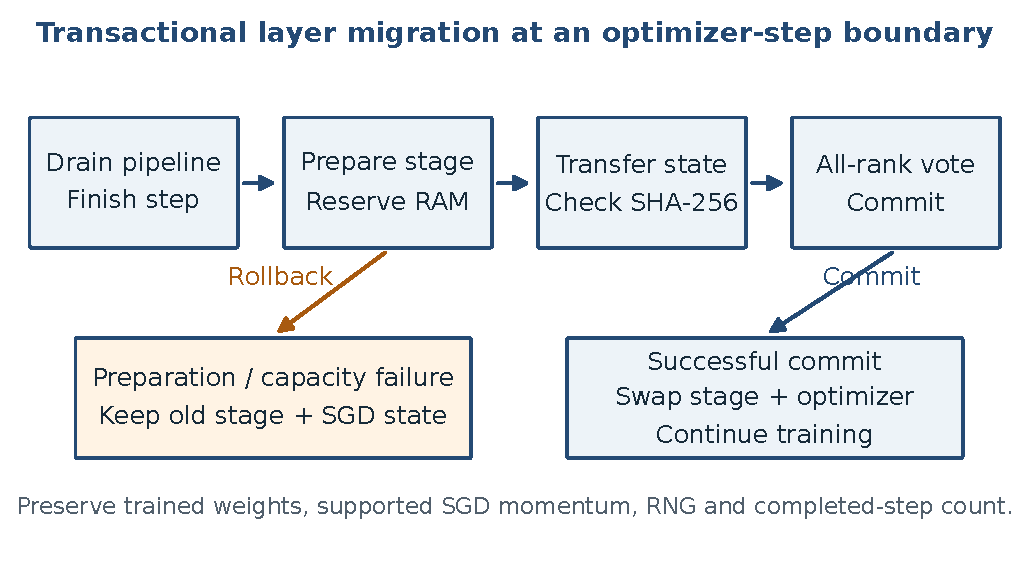
\includegraphics[width=\textwidth]{migration_transaction.pdf}
\caption{The implemented migration transaction retains the old stage until every rank can prepare and verify the replacement.}
\label{fig:migration}
\end{figure}

Layers have stable global identities. Only layers whose owner changes are transferred, with trained weights and supported optimizer state. Embeddings and the head remain at the endpoints. Receivers verify SHA-256 checksums and build candidate stages; all ranks vote before model and optimizer references are swapped. RNG state is preserved around profiling and migration, while the data iterator and completed-step count continue.

The transfer path supports FP32 SGD with one matching parameter group, including momentum buffers. Adam, mixed precision, arbitrary data-parallel groups and changing pipeline membership are outside this path. Preparation and capacity failures discard candidates and retain the old partition. A transport failure or crashed worker remains fatal.

Temporary storage is required because the old and candidate states coexist. The planner conservatively checks replacement and transfer headroom without assuming that old storage has already been freed. Thus, a proposed migration can be skipped even when its final partition would fit after replacement. This choice protects trained state during preparation.

\subsection{Metrics, Logging and MLflow}

Instrumentation records forward, backward, optimizer and synchronization timings, wall time, completed steps, final-microbatch loss and communication matrices. Scheduling plans and rebalance events are added to the rank metrics. Microbatch-level progress messages make a stalled forward or backward phase easier to locate, and log-hub/tee tools make distributed output easier to collect.

MLflow is optional. Each rank creates its own run, with a shared launch-group tag connecting one distributed job. Tracking stores workload parameters, step-indexed timings, throughput, endpoint loss and JSON artifacts. Run status reflects success or failure; one finished rank alone does not prove whole-job success. The multi-node guide supplies a central server arrangement, and the rank launcher adds connectivity checks and rank-0 server startup when tracking is configured.

For an input batch of size $b$ and measured iteration time $t$, the per-rank metric uses
\[
  \text{samples per second}=\frac{b}{t}.
\]
Pipeline ranks describe the same batch; their values must not be summed. Loss is the last microbatch's loss, not an average over the full batch. Forward/backward timers contain communication and waiting, and barrier timing can overlap them. These semantics are kept explicit in demonstrations and reports.

\subsection{Automated Lab Comparison and Reports}

The lab workflow coordinates two or three computers through an HTTP control service. Rank 0 supplies worker commands, coordinates trials, checks their consistency and automatically collects results. It compares equal allocation, measured-resource allocation and a standalone reference under fixed workload settings. Workers retain local training logs, and rank 0 creates a self-contained HTML report and a mentor ZIP.

The default three-rank workload has six transformer layers, sequence length 64, width 128, batch size 8, microbatch size 2 and FP32 SGD. Equal allocation is $2/2/2$. The workflow uses five warmup steps, 60 measured steps and three repetitions per configuration. Real-data trials use a fixed QQP subset; synthetic trials are explicitly labeled. The lab workflow does not enable mid-training migration.

The two-host path supports a $3/3$ equal split for the default model. A larger preset uses 12 layers, width 512, sequence length 128, eight heads, batch size 16 and microbatch size two, approximately 53 million parameters with the QQP vocabulary. It calibrates CPU threads and can compare both hosts' standalone baselines. This preset is CPU training; inventorying an installed GPU does not enable it automatically.

Reports include trial allocation, throughput, process wall time, stage timing, sampled memory, commands, configuration and hardware metadata. Incomplete, inconsistent or failed sessions are rejected rather than silently merged. Throughput uses the slowest rank's measured training window after warmup. Process-tree RSS is sampled every 100\,ms and can double-count shared pages; it is not exact peak GPU memory.

\subsection{Docker Deployment and Continuous Integration}

Docker packages training, profiling, scheduling, tracking and reporting tools. CPU and CUDA targets are supplied, and Compose includes single-worker, two-container pipeline and MLflow services. Datasets, cache and output are kept in persistent volumes or host mounts. Synthetic smoke tests do not require downloading QQP.

The published \texttt{suryanarayanaant/dtfm} repository has \texttt{cpu}, \texttt{cuda} and \texttt{latest} tags, confirmed on Docker Hub \cite{dockerhub}. Published images target Linux AMD64. The CPU target can also be built locally for ARM64. Containers do not replace host accelerator drivers or supply unsupported vendor runtimes; ROCm, XPU and DirectML native setups remain separate.

The CI workflow builds the CPU image, validates Compose, runs the existing tests and CPU smoke workloads, verifies completed steps across two containers, starts MLflow and runs its training demo. A separate job builds the CUDA image on a hosted runner without GPU execution. Saved measurement artifacts support inspection of the CPU jobs.

\subsection{Ongoing Application Extension: Tamil Summarization}

An additional workspace prototype introduces a separate two-rank encoder--decoder pipeline for \texttt{google/mt5-small} and the Tamil XL-Sum dataset \cite{mt5,xlsum}. Rank 0 owns the encoder and shared input embedding; rank 1 owns the decoder and output head. It uses CPU-staged Gloo, token-weighted gradient accumulation, Adafactor, distributed gradient clipping and final rank checkpoints. A utility assembles the two stages into a Hugging Face model directory.

This extension is present as uncommitted working-directory code at the reporting boundary. It is not included in the 36-commit count or the published 61-test CI result. It does not yet reuse the GPT layer scheduler or dynamic migration, and it supports exactly two pipeline ranks. No Tamil summarization quality or full pretrained-model multi-host result is claimed in this report.

% =============================================================================
\section{Experiments}
% =============================================================================

\subsection{Experimental Evidence and Interpretation}

Experiments are divided into four evidence types: published CI checks, recorded development verification, executable verification procedures and planned physical-host benchmarks. This prevents a documented command or planned configuration from being presented as a completed measurement. All numerical results below identify their scope.

\begin{table}[H]
\centering\small
\caption{Evidence sources used in this report.}
\begin{tabularx}{\textwidth}{P{2.9cm}YY}
\toprule
\textbf{Evidence} & \textbf{Source} & \textbf{Interpretation}\\
\midrule
Published automated checks & GitHub Actions run 37213825415 at commit \texttt{e0c0507}. & Current, reproducible CPU/container checks; CUDA image build only.\\
Recorded hardware verification & \texttt{SETUP.md}. & Development records for AMD and Intel UHD; physical mixed-host validation remains separate.\\
Recorded browser verification & \texttt{MLFLOW\_DEMO.md}, dated 15 September 2026. & Local CPU tracking, artifacts and browser behavior.\\
Migration-continuity checks & Test suite and \texttt{verify\_migration.py}. & Local CPU/Gloo state equivalence for live-rank transfers and injected preparation failures.\\
Lab workflow verification & \texttt{LAB\_DEMO.md}. & Real-data trials and reports on one development host; not three physical lab computers.\\
Planned deployment tests & Review 1 timeline and outstanding checks. & Test plan only; no measured WAN speedup or crash-recovery result.\\
\bottomrule
\end{tabularx}
\end{table}

\subsection{Single-Process and Local Pipeline Smoke Tests}

The standard CPU container workload uses a synthetic vocabulary of 512, sequence length 32, width 64, four attention heads, one layer per rank, batch size two and microbatch size one. It executes two real forward/backward/SGD iterations. The one-rank path includes embeddings, transformer layers and the task head in the same stage, resolving the original first/last-rank overlap for a single-process launch.

The local two-rank workload tests process-group initialization, activation transfer, backward-gradient return and optimizer execution. The latest CI also runs one rank per container on the Compose network and checks that each metrics file records the correct rank and two completed optimizer steps. This is stronger than checking that containers start, but it remains single-host execution.

The inherited NVIDIA setup includes one-process and two-process/one-GPU smoke scripts. Native vendor paths have separate environments, so a GPU result must identify the actual adapter, runtime and interpreter rather than infer execution from a successful CPU fallback.

\subsection{AMD and Intel UHD Development Verification}

The recorded Windows checks include single-process AMD ROCm training on a Radeon 860M and a local two-rank CPU/Radeon pipeline. The latter completed two full forward, backward and optimizer iterations over CPU-staged Gloo. This demonstrates compatible transport and autograd behavior for that local arrangement; it does not measure mixed-host network performance.

The recorded Intel UHD test used the Core i5-13450HX laptop under WSL, Python 3.11, PyTorch 2.4.1 and DirectML adapter index one. The integrated single-process smoke completed two SGD iterations and exited without the previously observed allocator problem. Reported final-microbatch loss changed from 1.0619 to 0.9157. A local CPU/Intel UHD two-rank test also completed two iterations and wrote both metrics files.

These observations establish device-path execution. Two iterations are insufficient to conclude convergence, and the timing difference between the first and later iteration includes initialization. Supported Intel XPU hardware still requires separate verification.

\subsection{Communication-Probe Failure Tests}

Probe tests cover rank-identity validation, directed aggregation, missing observations and consistency across ranks. The verification script starts two or three local CPU workers, performs network measurements and requires two completed training steps per rank. An additional case deliberately occupies one rank's probe port. Incoming measurements to that listener must remain \texttt{null}, while valid remaining links and training continue.

The recorded MLflow development verification also exercised this occupied-port case with three local ranks. The scenario concerns an unavailable auxiliary listener. It is not an experiment in recovering a killed training rank or a broken Gloo process group.

\subsection{Scheduled Launch and Resource-Pressure Checks}

Static scheduling checks validate model/profile compatibility, capacity limits, deterministic rank ordering, emitted shell commands and exact contiguous layer coverage. Dynamic checks validate shared memory accounting, one-layer feasibility, full-layer conservation and agreement between ranks. Controlled resource snapshots verify that pressure can change an allocation and that impossible allocations fail explicitly.

The launch verifier exercises training through emitted Bash commands rather than only inspecting manifest JSON. It checks rank topology, completed steps, stage counts, layer ranges and finite last-stage losses. Its network-order fixtures are synthetic; dynamic compute and memory readings can be live. Similar measured resources may correctly produce an equal split or no rebalance.

Example procedures available in the repository are:
\begin{lstlisting}
python scripts/verify_launch_manifest.py --scheduled --world-size 2
python scripts/verify_launch_manifest.py --dynamic --world-size 3 \
  --total-layers 7 --rebalance-every 1
\end{lstlisting}
These commands are reproducibility instructions. The report does not imply that every listed procedure was newly rerun during document preparation.

\subsection{Migration State-Continuity Experiment}

The migration experiment compares a fixed-partition baseline with explicit transfers, an injected candidate-construction failure and controller-driven allocation changes. Each case trains for four steps. The test assembles state by stable global layer identity and compares all final weights and nonempty SGD momentum buffers against the baseline. It also checks loss histories, RNG preservation and commit/rollback decisions.

This design verifies that transfers preserve the mathematical training state in the tested CPU/Gloo setting. An injected preparation failure must leave the old stage active and produce the expected rollback history. The current CI suite includes the two-rank continuity test. A separate verifier supports two or three local ranks, but physical multi-host and accelerator migration remain unvalidated.

\subsection{MLflow Tracking Demonstration}

The documented 15 September demonstration completed two single-rank CPU trials and one two-rank CPU/Gloo trial, with 20 optimizer iterations per rank. Four MLflow runs were verified as \texttt{FINISHED}. Step-indexed timings and throughput were checked, downloaded artifacts matched local JSON, and both pipeline ranks stored identical measured communication matrices.

An invalid model configuration produced a nonzero exit and a tracked \texttt{FAILED} run. Browser comparison showed both learning-rate configurations and loss curves through step 20. Final recorded losses for the two single-rank trials were 0.5496012568 and 0.7366819382. These are synthetic final-microbatch losses; they are not QQP accuracy or a distributed speedup comparison. The two-rank trial has a different total layer depth from the one-rank trials.

The latest Docker CI independently exercises a shorter two-step MLflow demonstration. It verifies the packaged tracking workflow; the earlier 20-step development record supplies the longer browser/artifact inspection.

\subsection{Real-Data Lab Workflow Verification}

The recorded Windows lab validation created a fresh environment, completed the setup script and two-process smoke test, and ran real QQP equal/resource/single trials through PowerShell with automatic reports. The Python launcher also completed two repetitions of each configuration. The workers were local processes on one development machine, so this verifies orchestration, data handling, training, collection and report generation.

A physical two/three-computer experiment must additionally verify peer reachability, consistent code and runtime versions, Gloo peer connections and the correct network interface. Opening only the rendezvous port is insufficient. The lab control service, probe and training peer traffic must all be reachable through the selected LAN or VPN.

\subsection{Fair Physical-Host Benchmark Protocol}

For the next benchmark, use the same total model, vocabulary, dataset subset, batch size, microbatch size, optimizer and measured-step budget in every configuration. Keep each host's calibrated CPU thread setting fixed. Record warmup separately, repeat trials and compare measured-resource allocation with equal allocation and the fastest measured standalone baseline.

The main system metric is end-to-end examples per second using the slowest rank's measured window. Also record total process wall time, allocation/calibration overhead, migration overhead where enabled, stage timings and sampled memory. Loss remains a training-objective check. A useful performance claim requires measured results with their repeat variability and hardware/network configuration, not a predicted scheduler bottleneck alone.

For migration, introduce controlled resource-pressure changes while all ranks remain alive, then check state and performance. Worker-loss recovery requires a different experiment after a recovery mechanism is implemented. Compression likewise requires byte-count, runtime and quality comparisons before a benefit can be claimed.

% =============================================================================
\section{Results}
% =============================================================================

\subsection{Latest Published CI Result}

GitHub Actions run \texttt{37213825415}, associated with commit \texttt{e0c0507}, completed successfully on 4 October 2026 \cite{ci}. Its test log reports \textbf{61 tests in 35.024 seconds, all passing}. Both the CPU and CUDA-build jobs succeeded. The CUDA job's name and workflow explicitly state that it performs no GPU execution on the hosted runner.

\begin{table}[H]
\centering\small
\caption{Latest published automated result at the report's committed baseline.}
\begin{tabularx}{\textwidth}{P{3.7cm}P{1.4cm}Y}
\toprule
\textbf{Check} & \textbf{Result} & \textbf{Meaning}\\
\midrule
Existing test suite & Pass & 61 tests; includes migration state-continuity and tracking checks.\\
CPU image build / Compose validation & Pass & Packaged environment and service configuration build successfully.\\
One-rank CPU smoke & Pass & Two actual forward/backward/optimizer steps.\\
Two local CPU ranks & Pass & Pipeline transport and training execute within one container.\\
Two-container pipeline & Pass & Both rank metrics confirm two completed steps over the Compose network.\\
MLflow server and training demo & Pass & Tracking service and packaged demo execute successfully.\\
CUDA image build & Pass & Build compatibility; actual GPU training is not covered by this job.\\
\bottomrule
\end{tabularx}
\end{table}

The CI result is stronger evidence of reproducibility than a source-only feature inventory, but it does not certify every native accelerator, physical network or large model. The ongoing mT5 workspace extension is outside this published result.

\subsection{Improvements over the Original Repository}

The original code already provides the research baseline, pipeline/data-parallel implementations and communication-aware scheduling experiments. Our improvements primarily make this baseline usable on accessible hardware, connect allocation to real launches, preserve live training state during reassignment and make results inspectable.

\begin{table}[H]
\centering\small
\caption{Team additions beyond the original upstream baseline.}
\begin{tabularx}{\textwidth}{P{2.5cm}Y}
\toprule
\textbf{Area} & \textbf{Added behavior / artifacts}\\
\midrule
Local reproduction & Complete single-stage path, setup/data scripts and one/two-rank smoke workflows.\\
Device portability & CPU, ROCm, XPU and DirectML selection/setup paths alongside retained CUDA support.\\
Heterogeneous transport & CPU-staged Gloo activations/gradients with local CPU/AMD and CPU/Intel UHD execution records.\\
Operational tooling & Portable rank launcher, Tailscale support, log hub/tee/merge tools and per-microbatch progress.\\
Measurements & Directed network matrices, robust aggregation, timing, throughput, loss and explicit missing-link handling.\\
Launch generation & Profile-driven rank ordering, host/device mapping and executable launch manifests.\\
Allocation & Static minimax layer counts and dynamic shared-budget resource planning.\\
Migration & Periodic planning, transactional layer transfer, state checksums and live-rank preparation rollback.\\
Tracking & Optional per-rank MLflow, central server instructions, startup/connectivity checks and browser demo.\\
Lab evaluation & Controlled QQP/synthetic comparisons, larger CPU preset and automated reports/ZIP artifacts.\\
Deployment & CPU/CUDA Docker targets, Compose services, published image configuration and CI.\\
\bottomrule
\end{tabularx}
\end{table}

\subsection{Development Milestones}

Figure~\ref{fig:progress} shows the cumulative commits after the original baseline. Commits include fixes, documentation and merges as well as feature work. The curve is a history measure, not a throughput or model-quality measure. Individual Git author counts are not used to infer task ownership for team members who are listed in the presentation but do not have matching commit identities.

\begin{figure}[H]
\centering
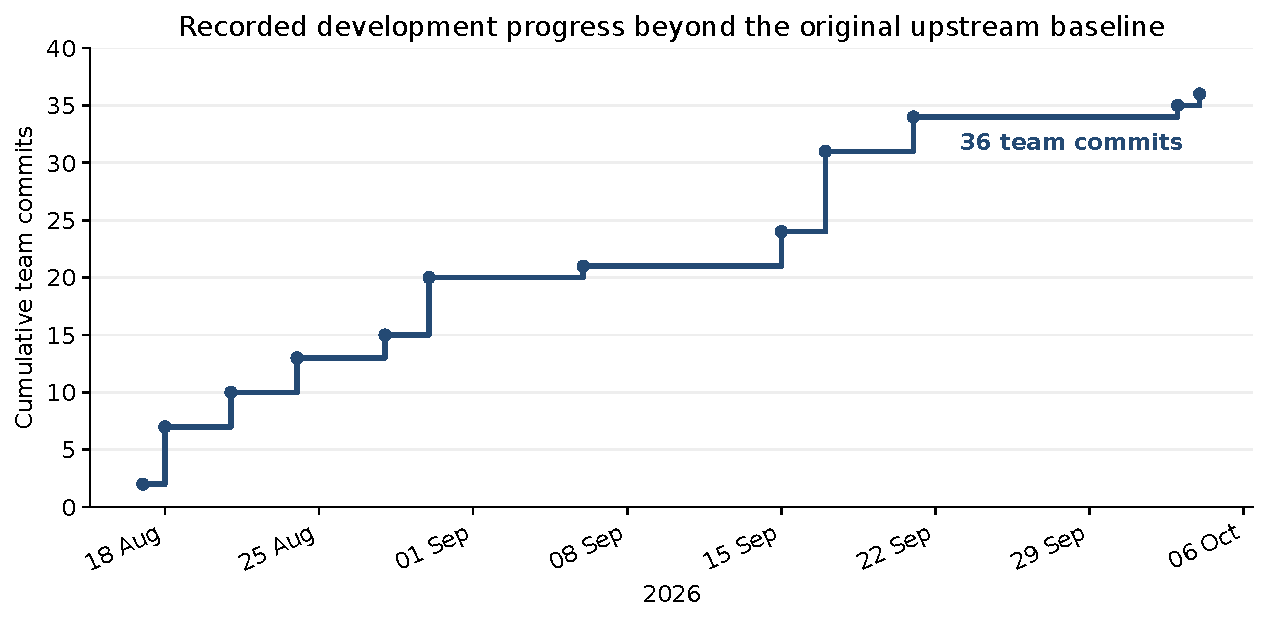
\includegraphics[width=0.96\textwidth]{development_progress.pdf}
\caption{Recorded team development history from 17 August to 4 October 2026: 36 commits beyond upstream.}
\label{fig:progress}
\end{figure}

\begin{table}[H]
\centering\small
\caption{Major implementation milestones from Git history.}
\begin{tabularx}{\textwidth}{P{2.55cm}Y}
\toprule
\textbf{Date} & \textbf{Recorded milestone}\\
\midrule
17--24 August & Local CUDA/QQP reproduction; setup compatibility, rank/log tooling, BERT-style presets, communication probes and progress diagnostics.\\
28--30 August & CPU/AMD, Intel XPU and Intel UHD DirectML support; mixed-device Gloo implementation and hardware execution records.\\
6 September & Probe aggregation and listener-failure handling corrections.\\
15 September & Optional MLflow, browser validation, profile-driven manifests and portable launcher.\\
17 September & Compute allocation, live resource discovery, migration/rebalancing, launch integration and continuity verification.\\
21 September & Multi-computer lab workflow and centralized MLflow/BERT-500M configuration.\\
3--4 October & Docker CPU/CUDA workflows, passing CI and published-image configuration/documentation.\\
\bottomrule
\end{tabularx}
\end{table}

\subsection{Current Completion Status}

The portable runtime, measurement tools, scheduling integration, migration transaction, experiment tracking, lab workflow and Docker packaging are implemented. The strongest continuously verified path is CPU/Gloo. AMD and Intel UHD have recorded local hardware results; Intel XPU awaits supported-device execution. The broader project is therefore at a functional prototype and reproducible local evaluation stage.

The published image tags allow users to run a small CPU workload without building the environment. The repository's \texttt{main} branch contains the latest documentation/configuration commit, while its default \texttt{master} branch is one commit behind at \texttt{dcb09b4}. This difference concerns the published-image instructions and configuration, not an uncommitted scheduler feature.

No supported evidence currently establishes WAN speedup, large-scale training quality, automatic recovery after worker loss or a compression benefit. A feature-completion percentage would hide these differences in validation scope and is therefore not assigned.

\subsection{Relationship to the Review 1 Timeline}

The supplied timeline spans July--November, covering problem formulation, literature review, baseline setup, system design, scheduler development, fault tolerance, communication optimization, testing and final documentation. Figure~\ref{fig:timeline} retains that plan. It should be read alongside the implementation milestones rather than treated as proof that all scheduled phases are complete.

\begin{figure}[H]
\centering
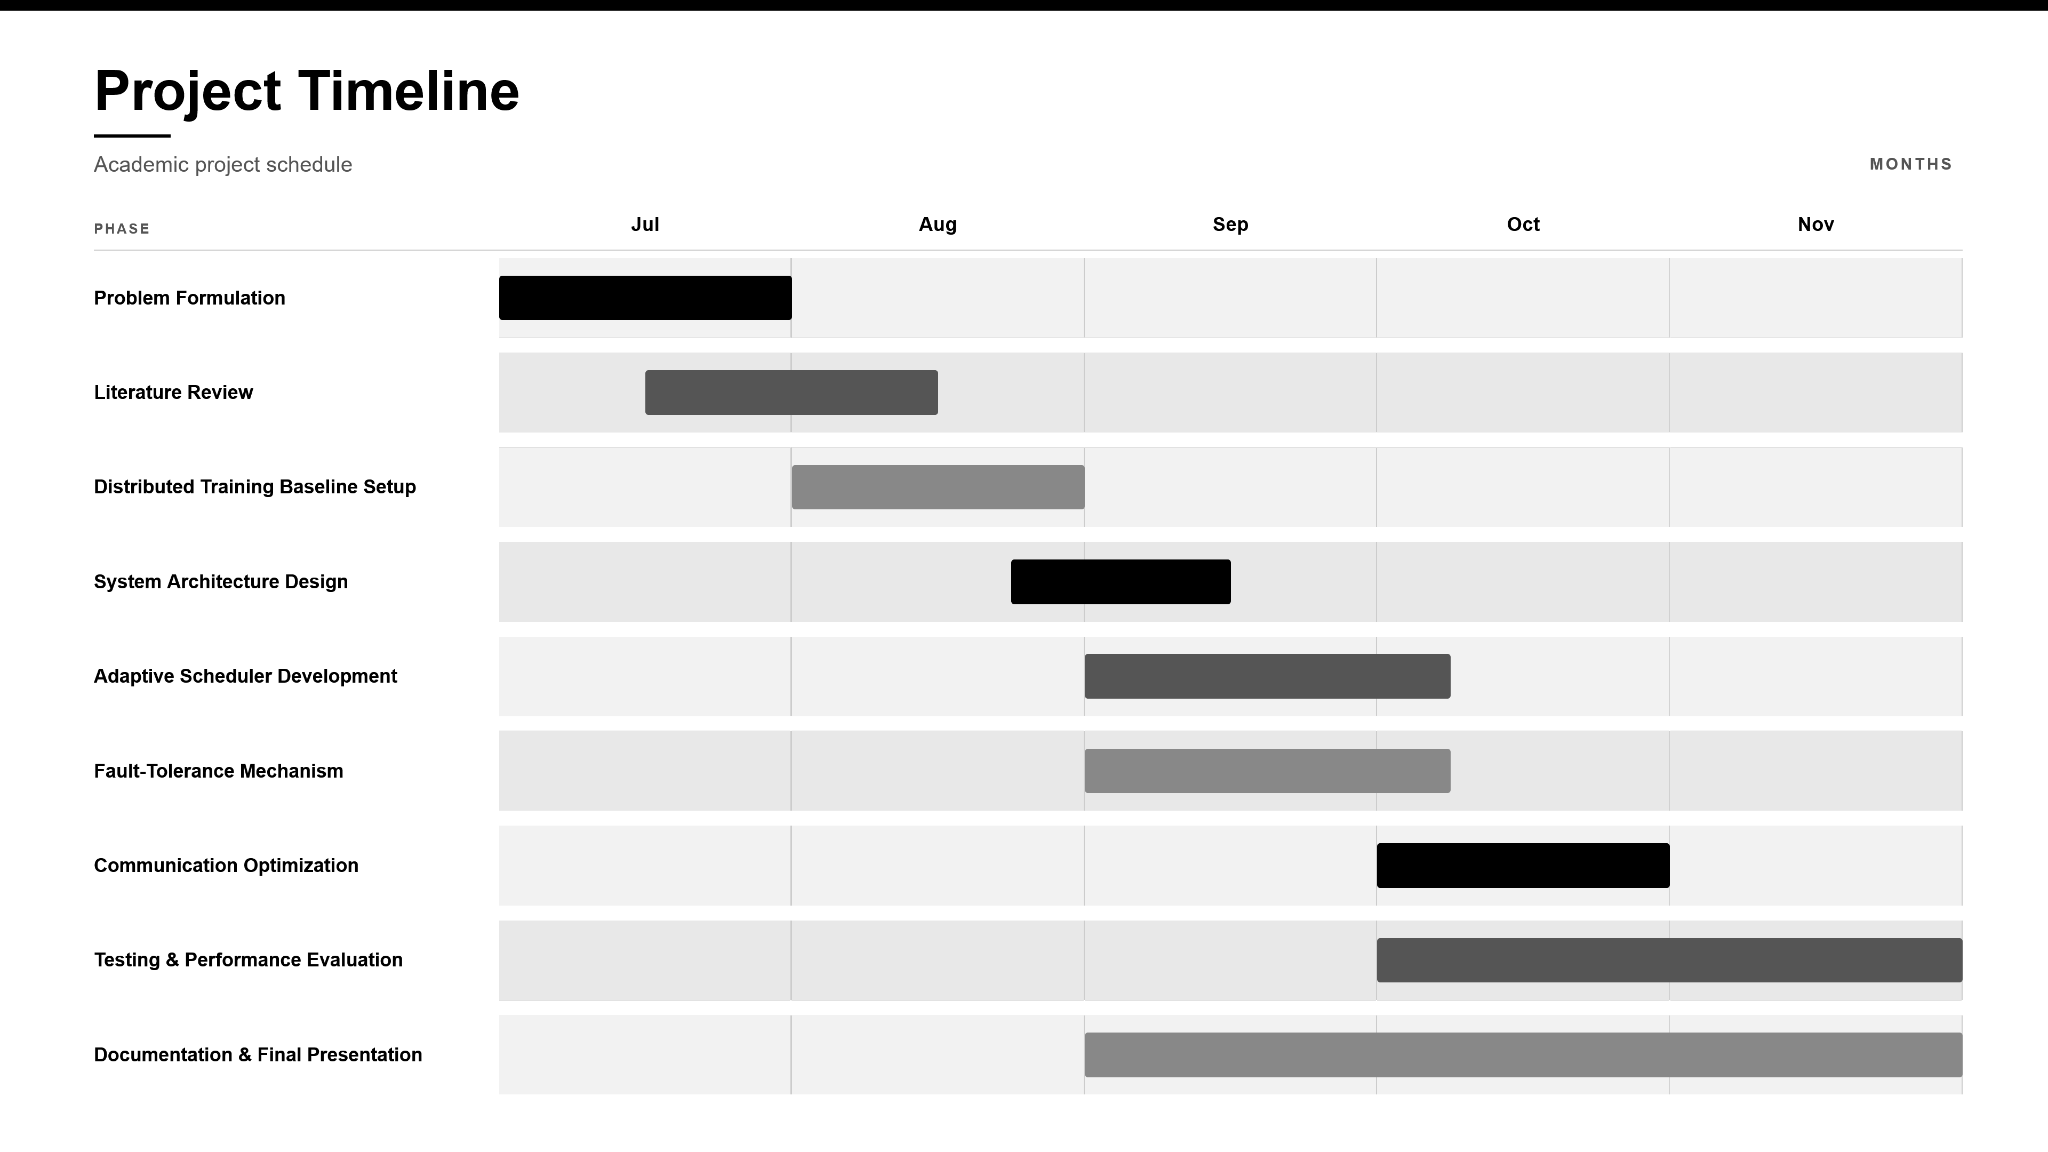
\includegraphics[width=\textwidth]{planned_timeline.png}
\caption{Planned academic project timeline reproduced from Review 1. This is the original plan, not a measured completion chart.}
\label{fig:timeline}
\end{figure}

Adaptive allocation and live-rank migration now have implementation evidence. The failure-recovery and compression phases remain future work, while physical-host performance testing must still establish whether the implemented scheduling produces a useful benefit under the intended network conditions.

% =============================================================================
\section{Conclusion}
% =============================================================================

The team has extended DT-FM from its original research-oriented baseline into a portable and observable training prototype. The central additions are multi-device runtime paths, CPU-staged heterogeneous pipelines, directed communication measurements, executable launch manifests, resource-aware contiguous layer allocation and state-preserving migration between live ranks. MLflow, automated lab comparisons and Docker deployment make these mechanisms easier to reproduce and inspect.

The latest published CI passes all 61 tests and demonstrates CPU training, two-container pipeline execution and the MLflow workflow. Recorded development checks additionally establish local AMD and Intel UHD execution and local CPU/Gloo migration continuity. These results support a concrete claim: the current system can construct, execute, measure and safely reassign supported pipeline work in the tested local arrangements.

The remaining project objective is to connect that functional correctness to measured benefit on physical heterogeneous hosts. Controlled comparisons must identify when unequal allocation improves throughput, how much profiling and migration cost, and how network conditions change the result. The proposed recovery and compression mechanisms require further implementation and independent evaluation. The current work provides the instrumentation and repeatable workflows needed to undertake those experiments without overstating the results already obtained.

% =============================================================================
\section{Limitations and Future Scope}
% =============================================================================

\subsection{Limitations}

\begin{enumerate}[leftmargin=1.1cm,itemsep=4pt]
  \item \textbf{Physical deployment evidence.} Local processes and containers do not establish physical multi-laptop or WAN operation. Network interfaces, peer ports and firewall behavior need validation on the intended hosts.
  \item \textbf{Performance evidence.} Compute estimates, successful execution and decreasing smoke loss do not establish distributed speedup. Controlled repeats and comparable standalone baselines remain necessary.
  \item \textbf{Model quality.} Synthetic smoke and short QQP trials are system checks. The main workflow does not produce held-out accuracy/F1, general foundation-model quality evidence or completed large-model convergence results.
  \item \textbf{Fixed training membership.} A lost rank or failed transport is fatal. Preparation rollback does not provide checkpoint recovery, elastic membership or automatic replacement of a crashed worker.
  \item \textbf{Migration scope.} The current path requires pipeline-only FP32 SGD with a matching parameter group. GPU and physical multi-host state migration remain to be verified; other optimizers and mixed precision are not covered.
  \item \textbf{Memory estimates.} Estimated activations/workspace and 25\% padding are not exact peaks. Other applications can change available memory after discovery, and candidate migration needs temporary headroom.
  \item \textbf{Device coverage.} Intel XPU needs a supported-hardware test. DirectML lacks dynamic free-memory discovery. Docker images do not include every native vendor runtime or replace host drivers.
  \item \textbf{Communication path.} CPU staging adds host copies and may limit throughput. The system does not currently implement compression or heterogeneous GPU-to-GPU collective communication.
  \item \textbf{Measurement semantics.} RTT and echo bandwidth are proxies. Timings include waiting, sampled RSS is approximate, and final-microbatch loss must not be interpreted as validation quality.
  \item \textbf{Application extension.} The uncommitted mT5 path is separate, supports exactly two ranks and does not inherit GPT scheduling/migration. Full pretrained-model training, multi-host execution and Tamil summary quality remain separate checks.
\end{enumerate}

\subsection{Future Scope}

The next priority is a reproducible two/three-host evaluation on the actual team or lab machines. Record hardware, runtime, interface, network measurements and workload configuration; compare equal allocation, resource allocation and the fastest standalone reference; retain all artifacts and repeat statistics. Then evaluate migration under controlled pressure and measure whether its benefit exceeds calibration and transfer overhead.

Supported Intel XPU execution and GPU migration should be verified independently. The allocator can then be extended with a cost model that combines computation, communication, pipeline behavior and migration cost rather than relying only on the present compute estimate.

Fault tolerance requires a defined failure detector, a source of recoverable trained state, consistent optimizer/data progress and a recovery protocol. ReCycle motivates using surviving redundant peers, but implementing such redundancy would change the present pipeline-only membership assumptions. Recovery must be tested with deliberately killed workers and transport failures, not only candidate-preparation exceptions.

Communication optimization should first quantify bytes transferred and host-copy overhead. Candidate gradient or activation compression methods need a defined error-handling scheme and comparisons of traffic, runtime, convergence and quality. An uncompressed baseline must remain available.

Finally, application-level evaluation can move beyond synthetic and small QQP workloads. The ongoing Tamil mT5 pipeline offers a concrete downstream direction once its deployment and full fine-tuning are verified. Held-out evaluation and generated-summary assessment should accompany system measurements. Final documentation should report successful, unsuccessful and unchanged allocations with the same experimental discipline.

\FloatBarrier
\newpage
\addcontentsline{toc}{section}{References}
\begingroup
\small
\setstretch{1.12}
\begin{thebibliography}{12}
\setlength{\itemsep}{5pt}

\bibitem{dtfm}
B. Yuan, Y. He, J. Q. Davis, T. Zhang, T. Dao, B. Chen, P. Liang, C. R\'e and C. Zhang,
``Decentralized Training of Foundation Models in Heterogeneous Environments,''
\textit{Advances in Neural Information Processing Systems}, 2022.
\url{https://arxiv.org/abs/2206.01288}.

\bibitem{recycle}
S. Gandhi, M. Zhao, A. Skiadopoulos and C. Kozyrakis,
``ReCycle: Resilient Training of Large DNNs using Pipeline Adaptation,''
\textit{ACM SIGOPS Symposium on Operating Systems Principles}, 2024.
\url{https://doi.org/10.1145/3694715.3695960}.

\bibitem{dgc}
Y. Lin, S. Han, H. Mao, Y. Wang and W. J. Dally,
``Deep Gradient Compression: Reducing the Communication Bandwidth for Distributed Training,''
\textit{International Conference on Learning Representations}, 2018.
\url{https://openreview.net/forum?id=SkhQHMW0W}.

\bibitem{upstream}
DS3Lab, \textit{DT-FM original source repository}, baseline commit \texttt{cda948f}.
\url{https://github.com/DS3Lab/DT-FM}.

\bibitem{fork}
Project team, \textit{DT-FM extended repository}, committed reporting baseline \texttt{e0c0507}.
\url{https://github.com/Mohanakumarp/DT-FM}.
Implementation records: \texttt{SETUP.md}, \texttt{SCHEDULER.md}, \texttt{LAUNCH\_MANIFEST.md},
\texttt{MLFLOW\_DEMO.md}, \texttt{MLFLOW\_BERT\_GUIDE.md}, \texttt{LAB\_DEMO.md} and \texttt{DOCKER.md}.

\bibitem{ci}
Project team, \textit{Docker continuous-integration run 37213825415}, 4 October 2026.
\url{https://github.com/Mohanakumarp/DT-FM/actions/runs/37213825415}.

\bibitem{dockerhub}
Project team, \textit{Published DT-FM CPU and CUDA images}, Docker Hub. Tags checked on 4 October 2026.
\url{https://hub.docker.com/r/suryanarayanaant/dtfm/tags}.

\bibitem{mt5}
Google, \textit{mT5-small model card}.
\url{https://huggingface.co/google/mt5-small}.

\bibitem{xlsum}
CSEBUET NLP, \textit{XL-Sum dataset repository}.
\url{https://huggingface.co/datasets/csebuetnlp/xlsum}.

\bibitem{presentation}
Project team, \textit{GPU Tasklet scheduling -- Review 1}, supplied presentation.
Source of project title, student names/roll numbers, proposal diagrams and planned timeline.
Guide name and department confirmed by the team for this report.

\bibitem{psg}
PSG College of Technology, \textit{Official institutional website and logo}.
\url{https://www.psgtech.edu/}.

\end{thebibliography}
\endgroup
\end{document}
